%%%%%%%%%%%%%%%%%%%%%%%%%%%%%%%%%%%%%%%%%%%%%%%%%%%%%%%%%%%%%%%%%%%%
%%%           Vorlage für eine Ausarbeitung an der DHBW          %%%
%%%                                                              %%%
%%%      Bereiche die bearbeitet werden müssen werden durch      %%%
%%%      einen solchen Kommentarblock eingeleitet und enden      %%%
%%%      mit der nächsten Trennlinie.                            %%%
%%%                                                              %%%
%%%      In dieser Datei müssen folgende Bereiche bearbeitet     %%%
%%%      werden:                                                 %%%
%%%      - Angaben zur Arbeit                                    %%%
%%%      - EIGENE KAPITEL EINFÜGEN                               %%%
%%%                                                              %%%
%%%      Benötigte Seiten und Verzeichnisse können unter         %%%
%%%      "Einführung und Verzeichnisse" ein- bzw. auskommentiert %%%
%%%      werden.                                                 %%%
%%%                                                              %%%
%%%%%%%%%%%%%%%%%%%%%%%%%%%%%%%%%%%%%%%%%%%%%%%%%%%%%%%%%%%%%%%%%%%%

\documentclass[a4paper,12pt]{article}
\usepackage[left=2.5cm,right=2.5cm,top=2.5cm,bottom=2.5cm,includehead]{geometry}      % Einstellungen der Seitenränder
\usepackage[english, ngerman]{babel}                                                  % deutsche Silbentrennung
\usepackage[utf8]{inputenc}                                                           % Umlaute
\usepackage[T1]{fontenc}													                                    % Umlaute auch richtig ausgeben
\usepackage{newtxtext,newtxmath}                                                      % Font = Times New Roman
\usepackage{hyperref}
\usepackage[nottoc]{tocbibind}
\usepackage{fancyhdr}
\usepackage{setspace}
\usepackage[backend=bibtex, citestyle=authoryear, bibstyle=authoryear]{biblatex}      % Bibliothek für Zitate
\usepackage{csquotes}                                                                 % Zusatzpacket für Zitate
\usepackage{amsmath}                                                                  % Zurücksetzen der Tabellen- und Abbildungsnummerierung je Sektion
\usepackage[labelfont=bf,aboveskip=1mm]{caption}                                      % Bild- und Tabellenunterschrift (fett)
\usepackage[bottom,multiple,hang,marginal]{footmisc}                                  % Fußnoten [Ausrichtung unten, Trennung durch Seperator bei mehreren Fußnoten]
\usepackage{graphicx}  
\graphicspath{{./images/}}                                                            % Grafiken
\usepackage[dvipsnames]{xcolor}                                                       % Farbige Buchstaben
\usepackage{wrapfig}                                                                  % Bilder in Text integrieren
\usepackage{enumitem}                                                                 % Befehl setlist (Zeilenabstand für itemize Umgebung auf 1 setzen)
\usepackage{listings}                                                                 % Quelltexte
\definecolor{commentgreen}{RGB}{87,166,74}                                            % Kommentar-Farbe für Quellcode
\lstset{numbers=left, numberstyle=\tiny, numbersep=8pt, frame=single, framexleftmargin=15pt, breaklines=true, commentstyle=\color{commentgreen}}
\usepackage{tabularx}                                                                 % Tabellen
\usepackage{multirow}                                                                 % Mehrzeilige Tabelleneinträge
\usepackage[addtotoc]{abstract}                                                       % Abstract
\usepackage[nohyperlinks, printonlyused, withpage]{acronym}                           % Abkürzungen
\usepackage{dirtree}                                                                  % Ordnerstruktur (z.B. für Anhang)
\usepackage{float}
\usepackage{pdfpages}

%%%%%%%%%%%%%%%%%%%%%%%%%%%%%%%%%%%%%%%%%%%%%%%%%%%%%%%%%%%%%%%%%%%%
%%%                      Angaben zur Arbeit                      %%%
%%%%%%%%%%%%%%%%%%%%%%%%%%%%%%%%%%%%%%%%%%%%%%%%%%%%%%%%%%%%%%%%%%%%
\def\vFirmenlogoPfad{}                  %% relativer Pfad Bsp.: images/Firmenlogo.png
\def\vDHBWLogoPfad{images/DHBW_logo.jpg}                          %% relativer Pfad Bsp.: images/DHBW_logo.jpg
\def\vUnterschrift{}                    %% Pfad zu Bild mit Unterschrift (für digitale Abgabe) Bsp.: images/Unterschrift.png

\def\vTitel{Software Engineering 2}                           %% 
\def\vUntertitel{}                      %% 
\def\vArbeitstyp{Hausarbeit}                      %% Projektarbeit/Seminararbeit/Bachelorarbeit
\def\vArbeitsbezeichnung{}              %% T1000/T2000/T3000

\def\vLB{Lukas Braun}
\def\vJB{Johannes Brandenburger}
\def\vDF{David Felder}
\def\vFG{Florian Glaser}
\def\vFH{Florian Herkommer}
\def\vPP{Phillipp Patzelt}
\def\vHS{Henry Schuler}
\def\vBS{Baldur Siegel}



\def\vAutor{\vJB, \vLB, \vDF, \vFG, \vFH, \vPP, \vHS, \vBS}                           %% Vorname Nachname
\def\vMatrikelnummer{}                  %% 7-stellige Zahl
\def\vKursKuerzel{TIT20}                     %% Bsp.: TIT20
\def\vPhasenbezeichnung{Theoriephasen}               %% Praxisphase/Theoriephase
\def\vStudienJahr{dritte}                     %% erste/zweite/dritte
\def\vDHBWStandort{Ravensburg}                    %% Bsp.: Ravensburg
\def\vDHBWCampus{Friedrichshafen}                      %% Bsp.: Friedrichshafen
\def\vFakultaet{Technik}                       %% Technik/Wirtschaft
\def\vStudiengang{Informatik}                     %% Informationstechnik/...
\def\vKurs{TIT20}                     %% IT/...

\def\vBearbeitungsort{Friedrichshafen}                 %%                       %% 
\def\vBetreuer{Prof. Dr. Andreas Judt}                        %% Vorname Nachname

\def\vAbgabedatum{\today}               %% DD. MONTH YYYY
\def\vBearbeitungszeitraum{01.10.2022 - 23.12.2022}            %% DD.MM.YYYY - DD.MM.YYYY
%TODO Datum anpassen

%%%%%%%%%%%%%%%%%%%%%%%%% Eigene Kommandos %%%%%%%%%%%%%%%%%%%%%%%%%
% Definition von \gqq{}: Text in Anführungszeichen
\newcommand{\gqq}[1]{\glqq #1\grqq}
% Definition von \gq{}: Text in Anführungszeichen
\newcommand{\gq}[1]{\glq #1\grq}
% Spezielle Hervorhebung von Schlüsselwörtern
\newcommand{\textOrdner}[1]{\texttt{#1}}
\newcommand{\textVariable}[1]{\texttt{#1}}
\newcommand{\textKlasse}[1]{\texttt{#1}}
\newcommand{\textFunktion}[1]{\texttt{#1}}
\newcommand{\newparagraph}{\newline \newline}
% Quellenangabe bei Bildern
\newcommand{\customcaption}[2]{\caption[#1]{ #1. #2.}}

%%%%%%%%%%%%%%%%%%%% Zitatbibliothek einbinden %%%%%%%%%%%%%%%%%%%%%
\addbibresource{./literatur/literatur.bib}


%%%%%%%%%%%%%%%%%%%%%%%% PDF-Einstellungen %%%%%%%%%%%%%%%%%%%%%%%%%
\hypersetup{
  bookmarksopen=false,
	bookmarksnumbered=true,
	bookmarksopenlevel=0,
  pdftitle=\vTitel,
  pdfsubject=\vTitel,
  pdfauthor=\vAutor,
  pdfborder={0 0 0},
	pdfstartview=Fit,
  pdfpagelayout=SinglePage
}


%%%%%%%%%%%%%%%%%%%%%%%% Kopf- und Fußzeile %%%%%%%%%%%%%%%%%%%%%%%%
\pagestyle{fancy}
\setlength{\headheight}{15pt}
\fancyhf{}
\fancyhead[R]{\thepage}


%%%%%%%%%%%%%%%%%%%%%%%%%%%%%% Layout %%%%%%%%%%%%%%%%%%%%%%%%%%%%%%
\onehalfspacing
\setlist{noitemsep}

\addto\captionsngerman{
  \renewcommand{\figurename}{Abb.}
  \renewcommand{\tablename}{Tab.}
}
\numberwithin{table}{section}                               % Tabellennummerierung je Sektion zurücksetzen
\numberwithin{figure}{section}                              % Abbildungsnummerierung je Sektion zurücksetzen
\renewcommand{\thetable}{\arabic{section}.\arabic{table}}   % Tabellennummerierung mit Section
\renewcommand{\thefigure}{\arabic{section}.\arabic{figure}} % Abbildungsnummerierung mit Section
\renewcommand{\thefootnote}{\arabic{footnote}}              % Sektionsbezeichnung von Fußnoten entfernen

\renewcommand{\multfootsep}{, }                             % Mehrere Fußnoten durch ", " trennen


%%%%%%%%%%%%%%%%%%%%%%%%%%%%% Dokument %%%%%%%%%%%%%%%%%%%%%%%%%%%%%

\begin{document}


%%%%%%%%%%%%%%%%%%% Einführung und Verzeichnisse %%%%%%%%%%%%%%%%%%%
\pagenumbering{Roman}

\begin{titlepage}
  \begin{minipage}{6in}
    \vspace*{-2cm}
    \centering
    \hspace{-2cm}
	\ifx\vFirmenlogoPfad\empty
	\else
    \raisebox{-0.5\height}{\includegraphics[height=4cm]{\vFirmenlogoPfad}}
  \fi
	\hfill
	\ifx\vDHBWLogoPfad\empty
	\else
   	\raisebox{-0.5\height}{\includegraphics[height=4cm]{\vDHBWLogoPfad}}
	\fi
  \end{minipage}
  \begin{center}
    \vspace*{0.5cm}
    \Huge\textbf{\vTitel}\\
		\ifx\vUntertitel\empty
		\else
			\Large\rm\vUntertitel\\
		\fi
		\vspace*{2cm}
		\Large\textbf{\vArbeitstyp}
		\ifx\vArbeitsbezeichnung\empty
		\else
			\textbf{\vArbeitsbezeichnung}
		\fi
		\\
		\normalsize
		über die \vPhasenbezeichnung\ des \vStudienJahr{n}\ Studienjahrs \\
		\vspace*{1cm}
		an der Fakultät für \vFakultaet\\
		im Studiengang \vStudiengang\\
		\vspace*{0.5cm}
		an der DHBW \vDHBWStandort\\
		\ifx\vDHBWCampus\empty
		\else
		Campus \vDHBWCampus\\
		\fi
		\vspace*{0.5cm}
		von\\
		\ifx\vAutor\empty
		\else
			\vAutor\\
		\fi
		\vspace*{1cm}
		\vAbgabedatum
		\vfill
  \end{center}
  \begin{tabular}{ll}
    Bearbeitungszeitraum:&\vBearbeitungszeitraum\\
    Kurs:&\vKurs\\
	  Dozent der Hochschule:&\vBetreuer\\
  \end{tabular}
\end{titlepage}
\newpage
\setcounter{page}{2}
% \thispagestyle{empty}
\section*{\Huge{Sperrvermerk}}

\addcontentsline{toc}{section}{Sperrvermerk}
gemäß Ziffer 1.1.13 der Anlage 1 zu §§ 3, 4 und 5  der Studien- und Prüfungsordnung für die Bachelorstudiengänge im Studienbereich Technik der Dualen Hochschule Baden-Würt­tem­berg vom 29.09.2017.\\

\noindent \gqq{Der Inhalt dieser Arbeit darf weder als Ganzes noch in Auszügen Personen außerhalb des Prüfungsprozesses und des Evaluationsverfahrens zugänglich gemacht werden, sofern keine anders lautende Genehmigung vom Dualen Partner vorliegt.}

\vfill
\leavevmode
\newline
\parbox{6cm}{\strut\centering \vBearbeitungsort, \vAbgabedatum\hrule\strut\centering\footnotesize Ort, Datum} 
\hfill
\ifx\vUnterschrift\empty
\parbox{6cm}{\strut\hspace{1pt} \vAbteilung\hrule\strut\centering\footnotesize Abteilung, Unterschrift}
\else
\parbox{6cm}{\strut\hspace{1pt} \vAbteilung, \parbox[b]{3cm}{\vspace{-10cm}\includegraphics[width=3cm]{\vUnterschrift}}\hrule\strut\centering\footnotesize Abteilung, Unterschrift}
\fi
\vspace{1cm}

\newpage
\thispagestyle{empty}
\section*{\Huge{Gender Erklärung}}

\addcontentsline{toc}{section}{Gendererklärung}
Aus Gründen der besseren Lesbarkeit wird in dieser Bachelorarbeit auf die gleichzeitige Verwendung der Sprachformen männlich,
weiblich und divers (m/w/d) verzichtet. Sämtliche Formulierungen gelten gleichermaßen für alle Geschlechter.
\newpage
\thispagestyle{empty}
\section*{\Huge{Selbstständigkeitserklärung}}

\addcontentsline{toc}{section}{Selbstständigkeitserklärung}
gemäß Ziffer 1.1.13 der Anlage 1 zu §§ 3, 4 und 5  der Studien- und Prüfungsordnung für die Bachelorstudiengänge im Studienbereich Technik der Dualen Hochschule Baden-Würt­tem­berg vom 29.09.2017.

\noindent Wir versichern hiermit, dass wir unsere Bachelorarbeit (bzw. Projektarbeit oder Studienarbeit bzw. Hausarbeit) mit dem Thema: 
\begin{center}
	\Large\textbf{\vTitel}
\end{center}
selbstständig verfasst und keine anderen als die angegebenen Quellen und Hilfsmittel benutzt haben. Wir versichern zudem, dass die eingereichte elektronische Fassung mit der gedruckten Fassung übereinstimmt.

\vfill
\leavevmode
\newline
\parbox{7cm}{\strut\centering \vBearbeitungsort, \vAbgabedatum\hrule\strut\centering\footnotesize Ort, Datum} 
\hfill
\parbox{7cm}{\strut\hspace{1pt} \hrule\strut\centering\footnotesize \vJB}
\newline
\vspace{1cm}
\newline
\parbox{7cm}{\strut\centering \vBearbeitungsort, \vAbgabedatum\hrule\strut\centering\footnotesize Ort, Datum} 
\hfill
\parbox{7cm}{\strut\hspace{1pt} \hrule\strut\centering\footnotesize \vLB}
\newline
\vspace{1cm}
\newline
\parbox{7cm}{\strut\centering \vBearbeitungsort, \vAbgabedatum\hrule\strut\centering\footnotesize Ort, Datum} 
\hfill
\parbox{7cm}{\strut\hspace{1pt} \hrule\strut\centering\footnotesize \vDF}
\newline
\vspace{1cm}
\newline
\parbox{7cm}{\strut\centering \vBearbeitungsort, \vAbgabedatum\hrule\strut\centering\footnotesize Ort, Datum} 
\hfill
\parbox{7cm}{\strut\hspace{1pt} \hrule\strut\centering\footnotesize \vFG}
\newline
\vspace{1cm}
\newline
\parbox{7cm}{\strut\centering \vBearbeitungsort, \vAbgabedatum\hrule\strut\centering\footnotesize Ort, Datum} 
\hfill
\parbox{7cm}{\strut\hspace{1pt} \hrule\strut\centering\footnotesize \vFH}
\newline
\vspace{1cm}
\newline
\parbox{7cm}{\strut\centering \vBearbeitungsort, \vAbgabedatum\hrule\strut\centering\footnotesize Ort, Datum} 
\hfill
\parbox{7cm}{\strut\hspace{1pt} \hrule\strut\centering\footnotesize \vPP}
\newline
\vspace{1cm}
\newline
\parbox{7cm}{\strut\centering \vBearbeitungsort, \vAbgabedatum\hrule\strut\centering\footnotesize Ort, Datum} 
\hfill
\parbox{7cm}{\strut\hspace{1pt} \hrule\strut\centering\footnotesize \vHS}
\newline
\vspace{1cm}
\newline
\parbox{7cm}{\strut\centering \vBearbeitungsort, \vAbgabedatum\hrule\strut\centering\footnotesize Ort, Datum} 
\hfill
\parbox{7cm}{\strut\hspace{1pt} \hrule\strut\centering\footnotesize \vBS}
\newpage
%\phantomsection
\newenvironment{keywords}{
	\begin{flushleft}
	\small	
	\textbf{
		\iflanguage{ngerman}{Schlüsselwörter}{\iflanguage{english}{Keywords}{}}
	}
}{\end{flushleft}}

% Deutsche Zusammenfassung
\begin{abstract}
	
\end{abstract}

% Schlüsselwörter Deutsch
\begin{keywords}
	
\end{keywords}


\selectlanguage{english}
% Englisches Abstract
\begin{abstract}

\end{abstract}

% Schlüsselwörter Englisch
\begin{keywords}

\end{keywords}


\selectlanguage{ngerman}
\newpage
\pdfbookmark[1]{\contentsname}{toc}
\tableofcontents
\newpage
\section*{Abkürzungsverzeichnis}
\addcontentsline{toc}{section}{Abkürzungsverzeichnis}
\begin{acronym}
  \acro{DHBW}[DHBW]{Duale Hochschule Ba\-den-\-Würt\-tem\-berg}
  \acroplural{DHBW}[DHBW]{Dualen Hochschule Ba\-den-\-Würt\-tem\-berg}
  \acro{AWS}[AWS]{Amazon Web Services}
\end{acronym}
\newpage
\listoffigures
\newpage
\listoftables
\newpage
\lstlistoflistings
\addcontentsline{toc}{section}{Listings}
\newpage
% \section*{Vorwort}
\addcontentsline{toc}{section}{Vorwort}
\newpage


%%%%%%%%%%%%%%%%%%%%%%%%%%%%% Kapitel %%%%%%%%%%%%%%%%%%%%%%%%%%%%%%
\pagestyle{fancy}
\fancyhead[L]{\nouppercase{\rightmark}}    % Abschnittsname im Header
\pagenumbering{arabic}

%%%%%%%%%%%%%%%%%%%%%%%%%%%%%%%%%%%%%%%%%%%%%%%%%%%%%%%%%%%%%%%%%%%%
%%%%                   EIGENE KAPITEL EINFÜGEN                  %%%%
%%%%%%%%%%%%%%%%%%%%%%%%%%%%%%%%%%%%%%%%%%%%%%%%%%%%%%%%%%%%%%%%%%%%
\section{Einleitung}

\section{Fachklassendiagramm}

\noindent Das folgende Fachklassendiagramm \autoref{fig:Fachklassendiagramm} zeigt die benötigten Klassen mit ihren
Kardinalitäten, Attributen und Operationen für die Umsetzung des \ac{aMRS}. Bei der Modellierung wurden Design Patterns
berücksichtigt, um eine Entkopplung der Komponenten zu verwirklichen. Durch die Entkopplung soll eine bessere
Wartbarkeit, Erweiterbarkeit und die Qualität der Software sichergestellt werden. \newline

\noindent Wie in \autoref{fig:Fachklassendiagramm} zu erkennen ist das System in zwei unabhängige Teilsysteme
untergliedert, welche nur über die Datenspeicherung verbunden sind. Diese nutzt das Repository Pattern, um eine
Entkopplung der Datenzugriffsschicht vom restlichen System zu ermöglichen. Über das Adapter Pattern ist eine
Schnittstelle zwischen Informationsportal und \ac{aMRS} geplant. Zum andern bietet \ac{aMRS} mit ihrer eigenen GUI die
Möglichkeit den im \#TODO autoref ... beschriebenen Bewertungsprozess durchzuführen. Dieser Prozess nutzt einen Adapter
zu einem externen OCR-System und diverse Validatoren, welche mithilfe des Iterator Pattern leicht an zukünftige
Kundenwünsche angepasst werden können.

\newpage

\begin{figure}[H]
    \centering
    \caption{Fachklassendiagramm} \label{fig:Fachklassendiagramm}
    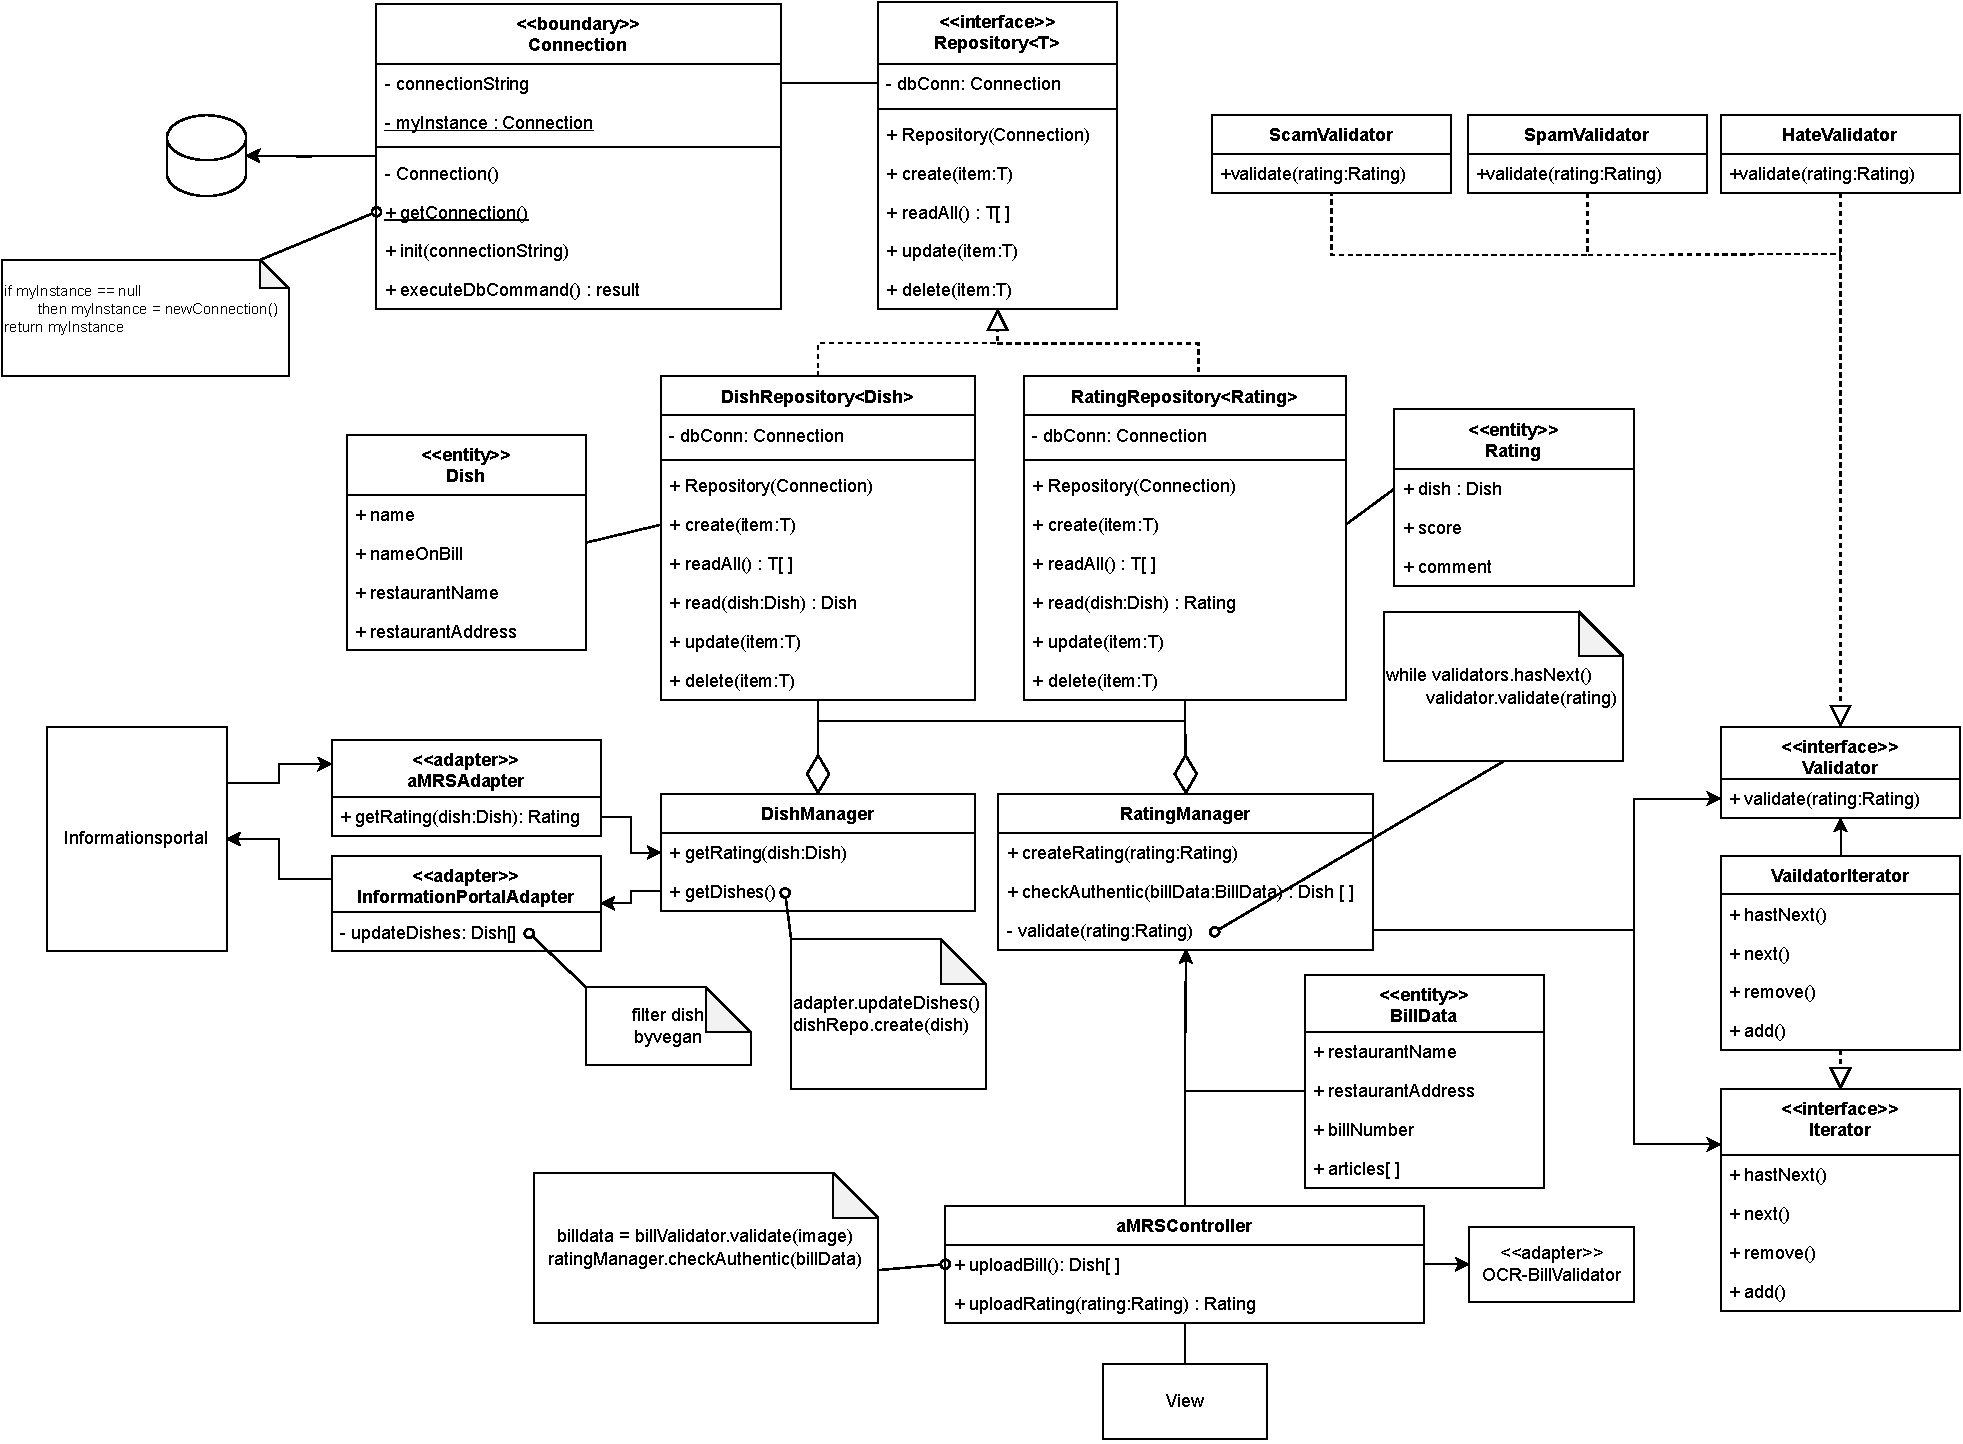
\includegraphics[width=1.3\textwidth,angle=90,keepaspectratio]{images/Fachklassenmodell}
\end{figure}

\section*{Beschreibung der Fachklassen}

\subsection*{Entity}
\textbf{Dish} \\
Die Klasse Dish enthält Informationen über Restaurantname, Restaurantadresse, Rechnungsbezeichner und Gerichtname des
Tagesgerichts.
\newline

\noindent \textbf{BillData} \\
Die Klasse BillData enthält Informationen über Restaurantname, Restaurantadresse, Rechnungsnummer und eine Liste aller
Rechnungsbezeichner der Restaurantrechnung.
\newline

\noindent \textbf{Rating} \\
Die Klasse Rating enthält Informationen über das zu bewertende Dish, eine Wertung und ein Kommentar.

\subsection*{Adapter}
\noindent \textbf{aMRSAdapter}\\
Die Klasse aMRSAdapter gitb dem Informationsportal die Möglichkeit Bewertungen vom \ac{aMRS} abzurufen.
\newline

\noindent \textbf{InformationsPortalAdapter}\\
Die Klasse InformationsPortalAdapter gitb dem \ac{aMRS} die Möglichkeit Tagesgerichte vom Informationsportal abzurufen.
Dabei werden die Tagesgerichte nach Klassifikation gefiltert.
\newline

\noindent \textbf{OCR-BillValidator}\\
Die Klasse OCR-BillValidator stellt die Kommunikation von \ac{aMRS} zum externen OCR-System her.


\subsection*{Boundary}
\noindent \textbf{Connection}\\
Die Klasse Connection empfängt Befehle zur Datenspeicherung beziehungsweise zum Datenzugriff.

\subsection*{Klasse}
\noindent \textbf{DishRepository<Dish>}\\
Die Klasse DishRepository ist für die Speicherung und den Zugriff auf die Daten der Klasse Dish zuständig.
\newline

\noindent \textbf{RatingRepository<Rating>}\\
Die Klasse RatingRepository ist für die Speicherung und den Zugriff auf die Daten der Klasse Rating zuständig.
\newline

\noindent \textbf{DishManager}\\
Die Klasse DishManager enthält die Logik für das Aktualisieren und Speichern neuer Dish-Objekte, sowie zum Abrufen von
vorhandenen Bewertungen.
\newline

\noindent \textbf{RatingManager}\\
Die Klasse RatingManager enthält die Logik für das Speichern und Validieren neuer Rating-Objekte. Zusätzlich wird das
Objekt BillData auf Authentizität überprüft.
\newline

\noindent \textbf{ScamValidator}\\
Die Klasse ScamValidator ist für die Überprüfung auf Scam in Bewertungen zuständig.
\newline

\noindent \textbf{SpamValidator}\\
Die Klasse SpamValidator ist für die Überprüfung auf Spam in Bewertungen zuständig.
\newline

\noindent \textbf{HateValidator}\\
Die Klasse HateValidator ist für die Überprüfung auf Hass in Bewertungen zuständig.
\newline

\noindent \textbf{ValidatorIterator}\\
Die Klasse ValidatorIterator ist für die Iteration über die Validatoren zuständig.
\newline

\noindent \textbf{aMRSController}\\
Die Klasse aMRSController ist für die Kommunikation zwischen View und RatingManager zuständig.
\newline

\noindent \textbf{View}\\
Die Klasse View stellt die GUI dar.

%%%%%%%%%%%%%%%%%%%%%%% Literaturverzeichnis %%%%%%%%%%%%%%%%%%%%%%%
\phantomsection
\addcontentsline{toc}{section}{Literatur}
\printbibliography
\newpage


%%%%%%%%%%%%%%%%%%%%%%%%%%%%%% Anhang %%%%%%%%%%%%%%%%%%%%%%%%%%%%%%
\renewcommand{\thetable}{\Alph{section}.\arabic{table}}
\renewcommand{\thefigure}{\Alph{section}.\arabic{figure}}
\renewcommand{\thelstlisting}{\Alph{section}.\arabic{lstlisting}}
\pagenumbering{Alph}

\begin{appendix}
  \section{Anhang}
\end{appendix}
\end{document}